\section{Data Analysis and Results}
% description of any analytically steps: parameter estimation, error estimation, model-fitting...



\subsection{Single Dish's Estimation of the Sun's Angular Diameter}

We  obtain a first estimative of the angular diameter of the Sun by comparing the Fourier components of the single dish measurements of the Sun and of the satellite. The size of the solar disk is the deconvolution of the single-dish solar profile with the single-dish satellite profile,
$$FFT(\Phi_{sun}^{Sin}) = \frac{FFT^{Sin}_{sun}}{FFT^{Sin}_{sat}},$$
resulting on the figure \ref{11}. We approximate the  central peak by a normal distribution and calculate the {\it full width at half maximum} (FWHM), as rough value for the  diameter of the Sun, $\Phi^{Sin}_{sun} \approx 25' $.


 \begin{figure}[htb]
\begin{center}
 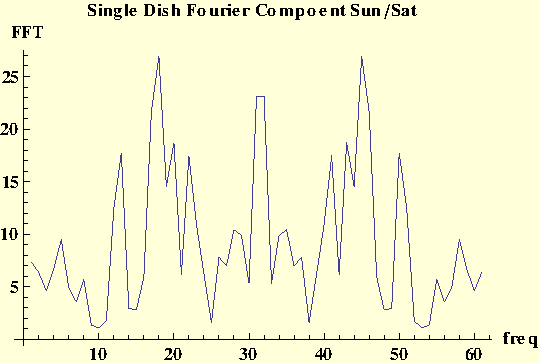
\includegraphics[scale=1.2]{plots/single.pdf}
\caption{The Sun's single dish Fourier component  over the satellite's. We  obtain a first calculation of the angular diameter of the Sun by calculating the FWHM of the central peak and Fourier transforming it. }
\label{11}
\end{center}
\end{figure}

\bigskip
\subsection{Calculation of the  Baselines  and Visibility Functions}
We calculate the baseline lengths for the set of five measurements of the Sun and of the satellite with the equation (\ref{BB}), converting the object's azimuth to the declination value, as in equation (\ref{dec}). The fringe frequency was numerically calculated by the Fourier transform profiles of the the total power data. The final values are shown in the table \ref{baselines} in the appendix.

From the same Fourier profiles we calculated the $P_{max}$ and $P_{min}$ points, as shown in the session \ref{visb}. The visibility functions are automatically obtained from the equation (\ref{vis}). 





\bigskip
\subsection{Obtaining the $\Phi_{sun}$ by Taylor-Approximating the Visibility Function} \label{taylormet}

The first method to estimate the value of the diameter of the sun is by plunging the values we have obtained for the visibility function into a Taylor approximation of the visibility equation (\ref{vissinc}),
$$ V_{sun}^{Tay}  = \frac{\sin(x)}{x} \approx \frac{x-x^3/6}{x} = 1 - \frac{x^2}{6}$$
where $x=\pi B_{\lambda} \Phi^{Tay}_{sun} $.

This gives  a value in radians for the  diameter of the Sun for one baseline, and it can later converted into arc minutes. A {\it Fast Fourier Transform} (FFT) of the fringe pattern shows a peak at the frequency of the fringe period $\Delta t$. Together with the equation (\ref{BB}), the angular diameter of the Sun can be calculated by
\begin{equation}
\Phi_{sun}^{Tay} = \frac{\sqrt{6}}{\pi} \frac{1}{B_{\lambda}} \sqrt{1 - V_{sun}^{Tay}(B_{\lambda})}.
\label{vistay}
\end{equation}

The mean and the standard deviation  for the five values obtained from this method results on $\Phi^{Tay}_{sun} = 37.43' \pm 5.33'$.



\bigskip

\subsection{Obtaining $\Phi_{sun}$ by Fitting the Fourier Components} \label{fitmet}


The second method to calculate the angular diameter of the sun is based on the fact that each measurement gives one Fourier component for baseline length. In the observations we obtain five Fourier components, $V_{sun}(B_{\lambda})$, which are a Fourier transformation of the energy density distribution, $\varepsilon(\theta_0)$. 

Plotting   $V_{sun}(B_{\lambda})$ vs. $B_{\lambda}$  exhibits  the Fourier transformation of the object structure. Since the structure of the Sun should be a {\it top-hat function}, the resulting plot (for its Fourier transformation) is exactly the {\it sinc function},
$$V^{fit}_{sun}(B_{\lambda}) = \mbox{ sinc }(B_{\lambda} {\Phi^{fit}_{sun}}),$$
 we saw in the equation (\ref{vissinc}). The sinc function sinc(x), also called the {\it sampling function} and  arises frequently in signal processing and the theory of Fourier transforms \cite{wiki}. 

We plot the Fourier components of the visibility function versus their baseline lengths, shown in the figure \ref{sing}. The fit gives the value of  $\Phi^{Fit}_{sun}= 32.77' \pm 5.28'$.




 \begin{figure}[htb]
\begin{center}
 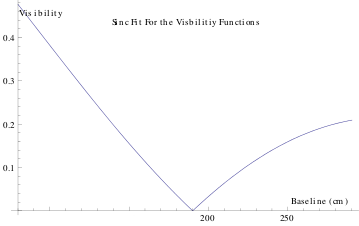
\includegraphics[scale=0.85]{plots/sinc3.png}
 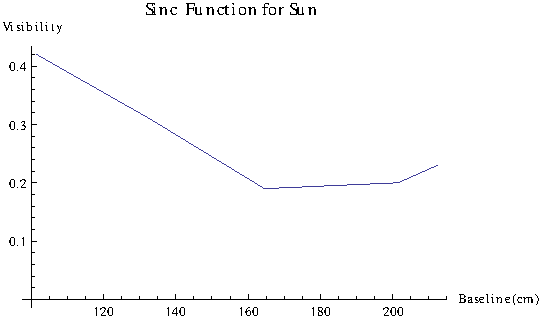
\includegraphics[scale=0.85]{plots/sinc1.pdf}
\caption{The Fourier components of the visibility function versus baselines, which is fitted by a sinc function, giving the value of the angular diameter of the sun. }
\label{sing}
\end{center}
\end{figure}



\bigskip
\subsection{Chi-Squared Fitting}
We use our knowledge of the {\it variance} (the measure of how far a set of numbers is spread out) of the measurements to fit it statistically by using the weighted sum of squared errors:
$$X^2 = \sum_i \frac{(O_i-E_i)^2}{\sigma_i^2}.$$

We assume that the variances, $\sigma^i$,  or our measurements are Gaussian functions and the the above equation will follow a {\it chi-squared distribution}. We obtain $\chi^2 = 12.3$ for the previous analysis.
